\documentclass[]{report}[12 pt]
\usepackage{geometry}
\usepackage{amsmath}
\usepackage{graphicx}
\usepackage{hyperref}
\geometry{margin= 1.5 cm}
\begin{document}
	\begin{titlepage}
	\begin{center}
		\vspace*{1cm}
		
		\Huge
		\textbf{Laboratory Report}
		
		\vspace{0.5cm}
		\LARGE
		X Ray Diffraction\\
		\vspace{0.5cm}
		\textbf{Guide: Prof. Sangita Bose}
		
		\vspace{1.5cm}
		
		\textbf{A R Bathri Narayanan}\\
		Roll no: P0211501\\
		UM DAE Centre for Excellence in Basic Sciences
		
		\vspace{3 cm}
		
		Report presented for the\\
		Advanced Physics Laboratory Course (PL 701)
		
		\vspace{0.8cm}
		
		
\includegraphics[width=0.4\textwidth]{cebs.jpg}
		
		\Large
		School of Physical Sciences\\
		UM-DAE Centre for Excellence in Basic Sciences\\
		Mumbai, MH, India\\
		\today
		
	\end{center}
\end{titlepage}
	\section*{Objectives:}

	\section*{Theory:}

	\section*{Observations:}
\subsection*{Finding the Resistance and Inductance of the given coil}
\subsection*{Detection of the Critical temperature of the chip}
We perform the experiment and get the critical temperature plots as follows
\begin{center}
	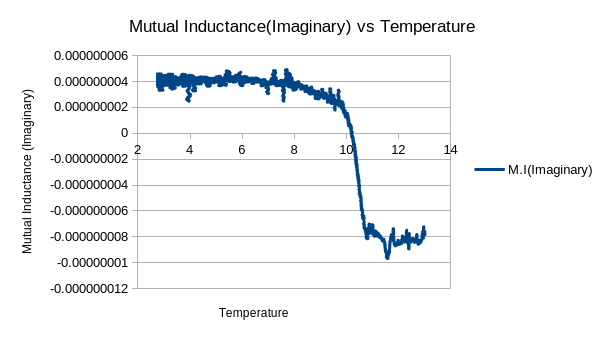
\includegraphics[width=11cm]{plot1.png}
	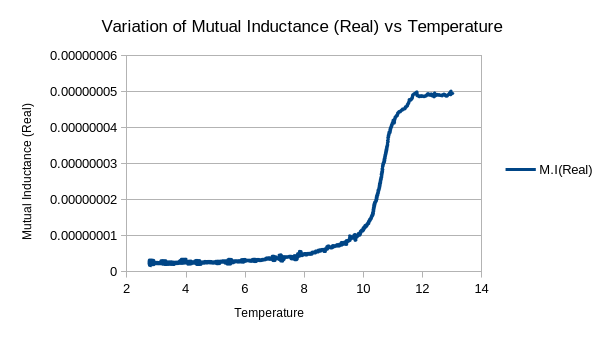
\includegraphics[width=11cm]{plot2.png}\\
	Plot of Mutual Inductance versus the temperature of both parts.
\end{center}
	We are getting the critical temperature of 10.213 K in the real part and 10.410K in the imaginary part. But then we were expecting a critical temperature of 11.2 K. What is more surprising is that there is some deviation in the real and imaginary values.
\end{document}